%--------------------------%
\section{January 2021} %---%
%--------------------------%
% \addcontentsline{toc}{section}{January 2021}

%%%%%%%%%%%%%%%%%%%%%%%%%%%%%%%%%%%%%
\subsection*{Classical Mechanics} %%%
%%%%%%%%%%%%%%%%%%%%%%%%%%%%%%%%%%%%%
\addcontentsline{toc}{subsection}{Classical Mechanics}

\prob{1.1}{

A smooth wire is bent into the shape of a spiral helix.
In cylindrical polar coordinates $(\rho,\phi,z)$ it is specified by equations $\rho = R \phi^2$ and $z = \lambda \phi^2$, where $R$ and $\lambda$ are constants and the $z$-axis is vertically up (and gravity vertically down).

\begin{parts}
    \item Using $z$ as your generalized coordinate, write down the Lagrangian for a bead of mass $m$ threadaed on the wire.

    \item Find the Lagrange equation and find from it the expression for the bead's vertical acceleration $\ddot{z}$ as a function of $z$ and $\dot{z}$.

    \item Find acceleration $\ddot{z}$ in two limits: (i) when $R \rightarrow 0$ but $\lambda$ is fixed, and (ii) when $\lambda \rightarrow \infty$ but $R$ is fixed.
    Discuss if the results for $\ddot{z}$ in these limits make sense.
\end{parts}

}

\sol{

We can write $x = \rho \cos{\phi}$ and $y = \rho \sin{\phi}$, so that
\begin{align}
    T = \frac{m}{2} (\dot{x}^2 + \dot{y}^2 + \dot{z}^2) = \frac{m}{2} ( \dot{\rho}^2 + \rho^2 \dot{\phi}^2 + \dot{z}^2 )
.\end{align}
Using the conditions, we have
\begin{align}
    \rho = \frac{R}{\lambda} z &\Rightarrow \dot{\rho} = \frac{R}{\lambda} \dot{z} \\
    \phi = \sqrt{\frac{z}{\lambda}} &\Rightarrow \dot{\phi} = \frac{\dot{z}}{2 \sqrt{\lambda z}}
.\end{align}
Thus
\begin{align}
    \eqbox{ L = \frac{m}{2} \Bigg[ \frac{R^2}{\lambda^2} \Bigg( 1 + \frac{z}{4 \lambda} \Bigg) + 1 \Bigg] \dot{z}^2 - m g z }
.\end{align}


(b) Next, we take derivatives to identify the equations of motion:
\begin{gather}
    \dv{t} \pdv{L}{\dot{z}} - \pdv{L}{z} = 0 \nonumber \\
    \eqbox{ \Bigg[ \frac{R^2}{\lambda^2} \Bigg( 1 + \frac{z}{4 \lambda} \Bigg) + 1 \Bigg] \ddot{z} + \frac{R^2}{8 \lambda^3} \dot{z}^2 + g = 0 }
.\end{gather}


(c) Finally, it is simple to take the limits prescribed:
\begin{gather}
    R \rightarrow \infty \Rightarrow \ddot{z} = -g \nonumber \\
    \lambda \rightarrow \infty \Rightarrow \ddot{z} = -g
\end{gather}

}


\prob{1.2}{

A particle with a mass $m$ and an orbital moment $L$ moves in an attractive potential which exerts a central force:
\begin{align*}
    \vb*{F} = - \frac{\alpha \vb*{r}}{r^3} e^{-r/R}
,\end{align*}
where $\alpha$ and $R$ are positive constants.
Show that a particle does not have stable circular orbits in this potential for $L > L_c$ and calculate the threshold value of $L_c$.

}

\sol{

There are two conditions for minima.
First, we need to have a point where the effective potential
\begin{align}
    U_{\rm eff} = \frac{L^2}{2 m r^2} + V(r)
\end{align}
is an extremum, and second, at that point, we must have that the potential is concave up.
For the first condition, we have
\begin{align}
    \dv{U_{\rm eff}}{r} = -\frac{L^2}{m r^3} + \dv{V}{r} = -\frac{L^2}{m r^3} - F(r) = 0 \Rightarrow r e^{-r/R} = \frac{L^2}{m \alpha}
.\end{align}
Note that the left-hand side is a function of $r$ which is strictly positive and has a maximum at $r = R$ of $R/e$, while the right-hand-side is a positive constant.
Therefore, if 
\begin{align}
    \eqbox{ L > \sqrt{m \alpha R / e} = L_c }
,\end{align}
there can be no stationary points on the effective potential.
We can now check that when solutions exist (i.e. $L < L_c)$, one of them yields a stable orbit:
\begin{align}
    \dv[2]{U_{\rm eff}}{r}\Big|_{r = r_0} &= \frac{3L^2}{m R^4} - \frac{\alpha}{r_0^3} \Big( 2 + \frac{r_0}{R} \Big) e^{-r_0/R} = \Bigg\{ \frac{3 r_0}{R^4} - \frac{1}{r_0^3} \Big( 2 + \frac{r_0}{R} \Big) \Bigg\} \alpha e^{-r_0/R} > 0 \nonumber \\
    &\Rightarrow 0 < r_0 < R
.\end{align}
One can easily check that $r_0 > R$ gives that $\dv*[2]{U_{\rm eff}}{r} |_{r_0=R} = 0$.


}


\prob{1.3}{

A massless inextensible string passes over a pulley located at a fixed distance above the floor.
A bunch of bananas of mass $m$ is attached at one end $A$ of the string.
A monkey of mass $M$ is initially at the other end $B$.
The monkey climbs the string, and his displacement $d(t)$ relative to the end $B$ is a given function of time.
The system is initially at rest, so that the initial conditions are $d(0) = \dot{d}(0) = 0$

\begin{parts}
    \item Introduce suitable generalized coordinates and obtain the Lagrangian in terms of these coordinates.

    \item Show that the equation of motion for the height $Z(t)$ of the monkey above the floor is given by
    \begin{align*}
        (m+M) \ddot{Z}(t) - m \ddot{d}(t) = (m-M) g
    .\end{align*}

    \item Integrate the differential equation to obtain the subsequent motion.

    \item In the special case $m = M$, show that the bananas and monkey rise through equal distances, so the vertical separation between them is constant.
\end{parts}

\begin{center}
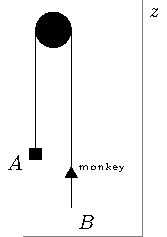
\includegraphics{January2021/1-3.pdf}
\end{center}

}

\sol{

(a) We can write the Lagrangian simply as
\begin{align}
    L = \frac{m \dot{z}_A^2}{2} + \frac{M \dot{Z}^2}{2} - m g z_A - M g Z
.\end{align}
At this point, we introduce the constraints relating the heights of the monkey and bananas, respectively, from the ground:
\begin{align}
    Z(t) = d(t) + z_B = d(t) - z_A + L \Rightarrow z_a = d - Z + L
,\end{align}
where $L = z_A + z_B$ is a constant.
From this, we write
\begin{align}
    \eqbox{ L = \frac{m ( \dot{d} - \dot{Z} )^2}{2} + \frac{M \dot{Z}^2}{2} - m g ( d - Z + L ) - M g Z }
.\end{align}


(b) We now use the Euler-Lagrange equation to find
\begin{gather}
    \dv{t} \pdv{L}{\dot{Z}} - \pdv{L}{Z} = -m (\ddot{d} - \ddot{Z}) + M \ddot{Z} - m g + M g = 0 \nonumber \\
    \Rightarrow \eqbox{ (m + M) \ddot{Z} - m \ddot{d} = (m - M) g }
\end{gather}

(c) We can integrate the above equation twice as follows
\begin{gather}
    (m + M) \dot{Z} - m \dot{d} = (m - M) g t \nonumber \\
    \eqbox{ Z(t) - Z_0 = \frac{m d(t) + (m - M) g t^2 / 2}{m + M} }
,\end{gather}
where we have assumed that the rope is initially stationary.


(d) If $m = M$, our equation of motion for $Z$ is
\begin{align}
    \ddot{Z} = \frac{\ddot{d}}{2} \Rightarrow \ddot{z}_A = \frac{\ddot{d}}{2}
.\end{align}
Thus, integrating twice, we have
\begin{align}
    \eqbox{ Z(t) - Z_0 = z_A - z_A(0) = \frac{d(t)}{2} }
.\end{align}
That is, the monkey's and banana's displacements from their initial positions are the same at all times $t > 0$.

}


\prob{1.4}{

A particle of mass $m$ moves in one dimension subject to the force
\begin{align*}
F = -kx + \frac{a}{x^3}
,\end{align*}
where both $k$ and $a$ are positive.

\begin{parts}
    \item What are the equilibrium points?
    Are they stable?

    \item Assume that the particle undergoes small oscillations around an equilibrium point.
    What are the frequency and period of the oscillations?

    \item Assume now that the total energy $E$ is large so that the small oscillations approximation is not valid.
    The motion is not sinusoidal anymore but it is still periodic.
    Show that the period of the oscillations is independent of the energy $E$ and therefore the period and frequency are still given by what was found in part (b).
\end{parts}

\textbf{Hint}: You may use the following integral:
\begin{align*}
    \int_a^b \frac{\dd{x}}{\sqrt{(x-a)(b-x)}} = \pi
\end{align*}

}

\sol{

(a) The equilibrium points are defined through
\begin{align}
    \dv{V}{x} = - F(x) = 0 \Rightarrow \eqbox{ x_{\pm} = \Big( \frac{a}{k} \Big)^{1/4} }
.\end{align}
We can determine if these are stable by considering
\begin{align}
    \dv[2]{V}{x} \Big|_{x = x_{\pm}} = -\dv{F}{x} = k + \frac{a}{x_{\pm}^4} = 4 k > 0
.\end{align}
Thus, these are stable equilibrium points.


(b) To find the period of small oscillations, we can Taylor expand our potential about these equilibria, yielding
\begin{align}
    V(x_{\pm}) = V(x_{\pm}) + \underbrace{ V'(x_{\pm}) }_{=0} (x - x_{\pm}) + \frac{V''(x_{\pm})}{2!} (x - x_{\pm})^2
.\end{align}
The leading order restoring force is a harmonic one such that the angular frequency and period of oscillation are given by
\begin{align}
    \eqbox{ \omega = \sqrt{\frac{V''(x_{\pm})}{m}} = 2 \sqrt{\frac{k}{m}} \Rightarrow T = \frac{2\pi}{\omega} = \pi \sqrt{\frac{m}{k}} }
,\end{align}
respectively.


(c) In this part, we use conservation of energy to write
\begin{align}
    T = \sqrt{2m} \int_{x_-}^{x_+} \frac{\dd{x}}{\sqrt{ E - V(x) }}
.\end{align}
The potential is given by $V(x) = [ k x^2 + a/x^2 ] / 2 = ( k x_0^2 / 2 ) [ (x/x_0)^2 + (x_0/x)^2 ]$, where we have used the fact that $a = k x_\pm^4$ and denoted $x_{\pm} = \pm x_0$.
Hence
\begin{align}
    T &= \sqrt{2m} \int_{a}^{b} \frac{\dd{x}}{\sqrt{ E - \frac{k x_0^2}{2} \Big[ (x/x_0)^2 + (x_0/x)^2 \Big]  }}
,\end{align}
where $a,b$ are defined such that $U(a) = U(b) = E$.
Let us introduce the substitution $u = ( x/x_0 )^2$
\begin{align}
    \eqbox{ T = \sqrt{\frac{m}{k}} \int_{(a/x_0)^2}^{(b/x_0)^2} \frac{\dd{u}}{\sqrt{\frac{2E}{k x_0^2} u - u^2 - 1}} = \sqrt{\frac{m}{k}} \int_{u_{-}}^{u_{+}} \frac{\dd{u}}{\sqrt{(u-u_{-})(u_+-u)}} = \pi \sqrt{\frac{m}{k}} }
,\end{align}
where
\begin{align}
    u_{\pm} = -\frac{E}{k x_0^2} \pm \sqrt{\Big( \frac{E}{kx_0} \Big)^2 - 1}
\end{align}
are the roots of the polynomial under the radical.
Notice that $u_{+} = (b/x_0)^2$ and $u_{-} = (a/x_0)^2$.

}


\prob{2.1}{

A particle of mass is subject to an attractive central force $\vb*{f}_1(\vb*{r}) = \vu*{r} f(r)$ and a frictional force $\vb*{f}_2(\vb*{r}) = -\lambda \vb*{v}$, where $\vb*{v}$ is the velocity of the particle and $\lambda > 0$.
The particle initially has an angular momentum $\vb*{L}_0$ about the origin.
By what time will the particle lose half of its angular momentum?

}

\sol{

Observe that
\begin{align}
    \dv{\vec{L}}{t} = \vec{r} \cross \vec{F} = \vec{r} \cross ( \vhat{r} f(r) - \lambda \vec{v} ) = -\lambda \vec{r} \cross \vec{v} = -\frac{\lambda}{m} \vec{L}
,\end{align}
which has solution
\begin{align}
    \vec{L}(t) = \vec{L}_0 e^{-(\lambda / m) t}
.\end{align}
Thus, the time $T$ elapsed such that $\vec{L}(T) = \vec{L}_0/2$ satisfies
\begin{align}
    \frac{1}{2} = e^{-(\lambda / m) T} \Rightarrow \eqbox{ T = \frac{m}{\lambda} \ln(2) } 
\end{align}

}


%%%%%%%%%%%%%%%%%%%%%%%%%%%%%%%%%%%%%%%%%%
\subsection*{Electricity \& Magnetism} %%%
%%%%%%%%%%%%%%%%%%%%%%%%%%%%%%%%%%%%%%%%%%
\addcontentsline{toc}{subsection}{Electricity \& Magnetism}


\prob{2.2}{

The largest world accelerator, LHC, is capable of accelerating protons up to the energy of 6.5 TeV, or approximately 7,000 times the rest energy of the proton.

\begin{parts}
    \item Find the difference $c - v = \delta v$ between the velocity $v$ of such a proton and the speed of light $c \approx 3 \times 10^8~{\rm m/sec}$.
    Find an analytic expression for $\delta v$ and only then substitute numbers.

    In fact, LHC is a collider in which two protons having this energy in the laboratory frame move towards each other (along, say, $x$-axis).

    \item Take the frame in which one of the protons is at rest.
    What is the velocity $v_2$ of the second proton in that frame?
    Since $v_2$ is very close to the speed of light, represent it as $v_2 = c - \delta v_2$, and find $\delta v_2$.
    Again, find an analytic expression for $\delta v_2$ and only then substitute numbers.

    \item What is the energy of the second proton in the rest frame of the first one?

    \item Imagine that we are in a rocket that leaves the Earth with the speed $v$ equal to the lab frame speed of the LHC protons.
    How far from the Earth (in light-years) would we find ourselves after spending 1 year of our life on such a rocket?
\end{parts}

}

\sol{

(a) For this part, we can compute $\gamma$ first:
\begin{align}
    \gamma = \frac{E}{mc^2} \approx 7000 \gg 1
.\end{align}
Then, we have
\begin{align}
    \gamma = \frac{1}{\sqrt{1 - \beta^2}} \Rightarrow \beta = \sqrt{1 - \frac{1}{\gamma^2}} = 1 - \frac{1}{2 \gamma^2} + \hdots
,\end{align}
so
\begin{align}
    \eqbox{ \delta v = c(1 - \beta) = \frac{c}{2 \gamma^2} \approx 3~{\rm m/s} }
.\end{align}

(b) Next, we can use the velocity addition rule to find
\begin{align}
    v_2 = \frac{2v}{1 + \beta^2} \Rightarrow \eqbox{ \delta v_2 = c(1 - \beta_2) = \frac{c}{8 \gamma^4} \approx 1.5 \times 10^{-8}~{\rm m/s} }
.\end{align}


(c) Here, we can simply use that
\begin{align}
    \eqbox{ E_2 = \gamma_2 m c^2 = \frac{m c^2}{\sqrt{1 - \beta_2^2}} = \frac{mc^2}{\sqrt{{\underbrace{(1 + \beta_2)}_{\approx 2} \underbrace{(1 - \beta_2)}_{=1/(8\gamma^4)}}}} = 2 \gamma^2 m c^2 \approx 10^{8}~{\rm GeV} }
.\end{align}

(d) Finally, we have that the distance the rocket travels in the frame of the earth is
\begin{align}
    \eqbox{ d = v t = \gamma v t' \approx \gamma c t' = 7000~{\rm lightyears} }
\end{align}

}


\prob{2.3}{

Two dipoles are a certain distance apart.
One is fixed at an angle $\varphi$ with the line joining the 2 dipoles.
The other is fixed in location but free to rotate and will be at an angle $\alpha$ with the same line.
What is the relationship between $\varphi$ and $\alpha$?

\begin{center}
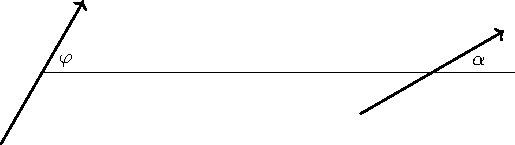
\includegraphics{January2021/2-3.pdf}
\end{center}

}

\sol{

The torque on the second dipole from the field of the first is just
\begin{align}
    \vec{N} &= \vec{p}_2 \cross \vec{E}_1(\vec{r_2}) = \vec{p_2} \cross \frac{3(\vec{p}_1 \cdot \vhat{n}) \vhat{n} - \vec{p}_1}{4 \pi \epsilon_0 r^3} \nonumber \\
    &= \frac{-p_1 p_2 [ 3 \cos{\varphi} \sin{\alpha} + \sin(\varphi - \alpha) ]}{4 \pi \epsilon_0 r^3} \vhat{z} = \frac{p_1 p_2 [ 2 \cos{\varphi} \sin{\alpha} + \sin{\varphi} \cos{\alpha} ]}{4 \pi \epsilon_0 r^3} \vhat{z}
,\end{align}
where I have chosen the $z$-axis to point out of the page.
At equilibrium, the torque is exactly zero, which imposes the condition that
\begin{gather}
    4 \cos{\varphi} \sin{\alpha} = -\sin{\varphi} \cos{\alpha} \Rightarrow \eqbox{ \tan{\alpha} = -\frac{1}{2} \tan{\varphi} }
\end{gather}

Alternatively, one could observe that the angle $\alpha$ is the same as that which the electric field makes with the axis at equilibrium, which is given by
\begin{align}
    \cos{\alpha} = \frac{2 \cos{\varphi}}{\sqrt{3 \cos^2{\varphi} + 1}}
.\end{align}
One can check that the results are equivalent (although there are some subtlelties related to the range of inverse trigonometric functions to be cautious of).
Also note that $\vec{p}$ can be either parallel to antiparallel to $\vec{E}$, so if $\alpha$ is a solution to either of the above equations, then $\alpha + n \pi$ also is for $n = \pm 1,2,\hdots$.

}


\prob{2.4}{

Show by explicit calculation that the energy of the classical system particles $+$ electromagnetic field given by (in Gaussian units)
\begin{align*}
    H = \sum_i \frac{1}{2} m_i \dot{\vb*{r}}_i^2(t) + \frac{1}{8 \pi} \int \dd[3]{\vb*{r}} \Big[ \vb*{E}^2(\vb*{r},t) + \vb*{B}^2(\vb*{r},t) \Big]
\end{align*}
is a constant of motion, namely
\begin{align*}
    \dv{H}{t} = 0
.\end{align*}
Here $\dot{\vb*{r}}(t)$ is the velocity of the particle.
Assume that the $\vb*{E}(\vb*{r},t)$ and $\vb*{B}(\vb*{r},t)$ fields vanish as $|\vb*{r}| \rightarrow \infty$.

\textbf{Hints}: You may need the expression for the current density given by
\begin{align*}
    \vb*{j}(\vb*{r},t) = \sum_i q_i \dot{\vb*{r}}_i(t) \delta[ \vb*{r} - \vb*{r}_i(t) ]
,\end{align*}
where $q_i$ is the charge of particle $i$.

}

\sol{

We will need Maxwell's equations in Gaussian units, which read as follows:
\begin{gather}
    \grad \cdot \vec{E} = 4 \pi \rho \\
    \grad \cross \vec{E} = -\frac{1}{c} \pdv{\vec{B}}{t} \\
    \grad \cdot \vec{B} = 0 \\
    \grad \cross \vec{B} = \frac{4 \pi}{c} \vec{j} + \frac{1}{c} \pdv{\vec{E}}{t}
.\end{gather}
Let us now take the derivative of the Hamiltonian:
\begin{align}
    \dv{H}{t} &= \sum_{i} m_i \dot{\vec{r}}_i \cdot \ddot{\vec{r}}_i + \frac{1}{4 \pi} \int \dd[3]{\vec{r}} \Big[ \vec{E} \cdot \dot{\vec{E}} + \vec{B} \cdot \dot{\vec{B}} \Big] \nonumber \\
    &= \sum_{i} m_i \dot{\vec{r}}_i \cdot \ddot{\vec{r}}_i + \frac{1}{4\pi} \int \dd[3]{\vec{r}} \Big\{ \vec{E} \cdot c \Big[ (\grad \cross \vec{B}) - \frac{4 \pi}{c} \vec{j} \Big] - \vec{B} \cdot c (\grad \cross \vec{E}) \Big\} \nonumber \\
    &= \sum_{i} m_i \dot{\vec{r}}_i \cdot \ddot{\vec{r}}_i + \frac{c}{4 \pi} \int \dd[3]{\vec{r}} \Big[ \vec{E} \cdot ( \grad \cross \vec{B} ) - \vec{B} ( \grad \cross \vec{E} ) \Big] - \int \dd[3]{\vec{r}} \vec{E} \cdot \vec{j} \nonumber \\
    &= \sum_{i} m_i \dot{\vec{r}}_i \cdot \ddot{\vec{r}}_i + \frac{c}{4 \pi} \int \dd[3]{\vec{r}} \grad \cdot (\vec{E} \cross \vec{B}) - \sum_i q_i \dot{\vec{r}}_i \cdot \vec{E}(\vec{r}_i)
.\end{align}
Observe that
\begin{align}Home
    \vec{F}_i = m_i \ddot{\vec{r}}_{i} = q_i \Big[ \vec{E}(\vec{r}_i) + \frac{\dot{\vec{r}}_i}{c} \cross \vec{B}(\vec{r}_i) \Big] \Rightarrow m_i \dot{\vec{r}}_i \cdot \ddot{\vec{r}}_i = q_i \dot{\vec{r}}_i \cdot \vec{E}(\vec{r}_i)
,\end{align}
so the first and last terms in our expansion cancel.
Thus,
\begin{align}
    \eqbox{ \dv{H}{t} = \frac{c}{4 \pi} \int \dd[3]{\vec{r}} \grad \cdot (\vec{E} \cross \vec{B}) = \oint \dd{\vec{S}} \cdot (\vec{E} \cross \vec{B}) = 0 }
\end{align}
since the fields go to zero at infinity.

}


\prob{3.1}{

A conducting sphere of radius $R_1$ carries charge $Q$.
A second, initially uncharged conducting sphere of radius $R_2$ is placed at large distance $R \gg R_1, R_2$ and then connected to the first sphere by a long thin wire with large resistance.
After a long time, the system of two conducting spheres reaches equilibrium.

\begin{parts}
    \item Find the electrostatic force between two spheres.

    \item Find the ohmic heat dissipated in the wire and the spheres.
    Neglect effects of radiation.
\end{parts}

}

\sol{

(a) Using Ohm's law, we see that at equilibrium no current flows and therefore that the potential difference between the spheres is zero:
\begin{align}
    V = \frac{1}{4 \pi \epsilon_0} \Bigg[ \frac{Q_1}{R_1} - \frac{Q_2}{R_2} \Bigg] = 0
,\end{align}
where we have used the assumption that $R \gg R_1,R_2$ to neglect the contributions to the potential from the other sphere at the surface of the other one.
Thus, we have the following system of equations at equilibrium:
\begin{align}
    \begin{cases}
        Q_1/R_1 - Q_2/R_2 = 0 \\
        Q_1 + Q_2 = Q
    \end{cases}
    \Rightarrow \begin{cases}
        Q_1 = Q [R_1 / (R_1 + R_2)] \\
        Q_2 = Q [R_2 / (R_1 + R_2)]
    .\end{cases}
\end{align}
From this, we calculate simply the magnitude of the force (clearly it is repulsive) between spheres using Coulomb's law:
\begin{align}
    \eqbox{ F = \frac{1}{4 \pi \epsilon_0} \frac{Q_1 Q_2}{R^2} = \frac{1}{4 \pi \epsilon_0} \frac{Q^2}{R^2} \frac{R_1 R_2}{(R_1 + R_2)^2} }
.\end{align}


(b) Finally, we can compute the heat dissipated while the spheres were approaching equilibrium as the difference between the energies of the configurations before the wire was connected and after equilibrium is achieved.
Observe that for a sphere with total charge $q$ and radius $r$ the energy stored in its field is
\begin{align}
    U = \frac{\epsilon_0}{2} \int \dd[3]{\vec{r}'} \vec{E}^2 = \frac{\epsilon_0}{2} \frac{q^2}{(4 \pi \epsilon_0)^2} \int \dd{\Omega'} \int_{r}^{\infty} \frac{\dd{r'}}{r'^2} = \frac{q^2}{2(4 \pi \epsilon_0) r}
.\end{align}
Thus, the energy dissipated to achieve equilibrium is
\begin{align}
    \mathcal{E} &= \frac{Q^2}{2(4 \pi \epsilon_0) R_1} - \Bigg[ \frac{Q_1^2}{2(4 \pi \epsilon_0) R_1} + \frac{Q_2^2}{2(4 \pi \epsilon_0) R_2} \Bigg] \nonumber \\
    &= \frac{Q^2}{2(4 \pi \epsilon_0)} \Bigg[ \frac{1}{R_1} - \Bigg( \frac{R_1}{(R_1 + R_2)^2} + \frac{R_2}{(R_1 + R_2)^2} \Bigg) \Bigg] \nonumber \\
    &= \eqbox{ \frac{Q^2}{2(4 \pi \epsilon_0)} \frac{R_2}{R_1(R_1 + R_2)} }
.\end{align}
Observe three limiting cases: $R_2 \ll R_1$ yields $\mathcal{E} \rightarrow 0$; $R_1 = R_2$ yields $\mathcal{E} = U_0/2$ (where $U_0$ is the energy of the initial configuration); and finally, $R_2 \gg R_1$ yields $\mathcal{E} \rightarrow U_0$.

}


\prob{3.2}{

Two identical electric dipoles rotate with a circular frequency $\omega$ in the same direction in the $xy$-plane.
The moment $\vb*{d}_2(t)$ of the second dipole makes a constant angle $\alpha$ with $\vb*{d}_1(t)$ of the first dipole, and $|\vb*{d}_1(t)| = |\vb*{d}_2(t)| = d_0$.
Calculate the net power of radiation $P_\omega$ as functions of $\omega$ and $\alpha$ if the spacing between the dipoles in the $xy$-plane is much smaller than the wavelength $2 \pi c / \omega$ of radiation.
Find the angles $\alpha_1$ and $\alpha_2$ at which $P_\omega$ is minimum and maximum, respectively.

\textbf{Hint}: The net power of dipole radiation is $P_\omega = 2 | \ddot{\vb*{d}} |^2 / (3c^2)$.

}

\sol{

The full dipole moment is just the sum $\vec{d} = \vec{d}_1 + \vec{d}_2$.
Since the dipole moments are rotating with frequency $\omega$, we have $\ddot{\vec{d}} = \omega^2 \vec{d}$ (to see this create a physical dipole where the charges are rotating and see what this implies about the dipole moment's time derivative).
Thus
\begin{align}
    \eqbox{ P_{\omega} = \frac{2 \omega^4 |\vec{d}_1 + \vec{d}_2|^2}{3 c^2} = \frac{2 \omega^4 \big[ |\vec{d}_1|^2 + 2 | \vec{d}_1 \cdot \vec{d}_2 | + |\vec{d}_2|^2 \big] }{3 c^2} = \frac{4 d_0^2 \omega^4 [1 + \cos{\alpha}]}{3 c^2} }
.\end{align}
Observe that if we restrict $\alpha \in [0,\pi]$, then a minimum in the net dipole radiation occurs when $\alpha_1 = \pi$ (i.e. when the dipoles cancel).
On the other hand, a maximum in the net dipole radiation occurs when $\alpha_2 = 0$ (i.e. when the dipoles sum to twice their strength).

}


%%%%%%%%%%%%%%%%%%%%%%%%%%%%%%%%%%%
\subsection*{Quantum Mechanics} %%%
%%%%%%%%%%%%%%%%%%%%%%%%%%%%%%%%%%%
\addcontentsline{toc}{subsection}{Quantum Mechanics}


\prob{3.3}{

Consider a spin-1/2 particle in one dimension subject to the spin-dependent interaction given by
\begin{align*}
    V(x) = V_0 \sigma_x \delta(x), \quad V_0 > 0
,\end{align*}
where $\delta(x)$ is the $\delta$-function at the origin and $\sigma_x$ is the Pauli matrix
\begin{align*}
    \sigma_x = \begin{pmatrix}
        0 & 1 \\
        1 & 0
    \end{pmatrix}
.\end{align*}
Assume the particle approaches the interaction region from the far left ($x = -\infty$) and has energy $E > 0$ and spin projection $+\hbar/2$ in the $\vu*{z}$-direction.
What is the probability that the particle has spin projection $-\hbar/2$ relative to the $\vu*{z}$-direction after it has traversed the interaction region and is at the far right ($x = \infty$)?

\textbf{Hint}: In the basis of eigenstates of $\sigma_x$ the Schr\"{o}dinger equation for spin up and spin down along the $\vu*{x}$-direction decouple.

}

\sol{

The relevant energy eigenvalue equation reads
\begin{align}
    \dv[2]{\ket{\Psi}}{x} + \Big[ k^2 - v_0 \sigma_x \delta(x) \Big] \ket{\Psi}
,\end{align}
where $v_0 = 2 m V_0 / \hbar^2$ and $E = \hbar^2 k^2 / (2m) > 0$.
Notice that if we consider the regions $x < 0$ and $x > 0$ separately, the particle is free
\begin{align}
    \ket{\Psi} = \begin{cases}
        e^{i k x} \ket{+} + e^{-ikx} ( A \ket{+}_{x} + B \ket{-}_{x} ) & x < 0 \\
        e^{ikx} ( C \ket{+}_{x} + D \ket{-}_{x} ) & x > 0
    .\end{cases}
\end{align}
Note that $\ket{+} = (\ket{+}_x + \ket{-}_x)/\sqrt{2}$.

We have two boundary conditions:
\begin{align}
    \ket{\Psi(x=0^{-})} = \ket{\Psi(x=0^{+})} &\Rightarrow 
    \begin{cases}
        \frac{1}{\sqrt{2}} + A = C \\
        \frac{1}{\sqrt{2}} + B = D
    \end{cases}
    \\
    \dv{\ket{\Psi(x=0^{+})}}{x} - \dv{\ket{\Psi(x=0^{-})}}{x} = v_0 \sigma_x \ket{\Psi(x=0)} &\Rightarrow 
    \begin{cases}
        ik [ C - \frac{1}{\sqrt{2}} + A ] = v_0 C \\
        ik[ D - \frac{1}{\sqrt{2}} + B ] = -v_0 D
    .\end{cases}
\end{align}
Observe that each boundary condition yields two equations since $\ip{+}{-} = 0$.
Solving these yields
\begin{align}
    A = -\frac{i}{\sqrt{2}(2 \alpha + i)}, \quad C = \frac{\sqrt{2} \alpha}{2 \alpha + i}, \quad B = \frac{i}{\sqrt{2}(2 \alpha - i)}, \quad D = \frac{\sqrt{2} \alpha}{2 \alpha - i}
,\end{align}
where $\alpha = k / v_0$.

Finally, we want the probability that a transmitted particle at $x = \infty$ is measured to have spin $-\hbar/2$, given by
\begin{align}
    \eqbox{ T_{\rm flip} = \Big| \frac{C - D}{\sqrt{2}} \Big|^2 = \Big| \frac{\alpha}{2 \alpha + i} - \frac{\alpha}{2 \alpha - i} \Big|^2 = \frac{4 \alpha^2}{(1 + 4 \alpha^2)^2} }
.\end{align}


}


\prob{3.4}{

Consider two identical spin-1/2 fermions each with mass $m$ confined to move along a line of length $L$.
The confining potential energy is zero for $L > x > 0$ and infinite elsewhere.

\begin{parts}
    \item What is the ground-state energy of the combined system?
    Write down the normalized ground-state wave function accounting for spatial and spin-state symmetry.

    \item What is the first excited energy level and its degeneracy?
    Write down the corresponding normalized wave functions.
\end{parts}

}

\sol{

(a) The Hamiltonian of our system reads
\begin{align}
    H = H_1 + H_2
,\end{align}
where $H_1$ and $H_2$ are the single infinite potential well Hamiltonians for particles 1 and 2, respectively.
The eigenstates of this combination are simply
the states $\ket{\Psi_{n_1 n_2, sm}} = \Psi_{n_1,n_2}(x)\ket{sm}$ (corresponding to energies $E = E_{n_1} + E_{n_2}$), where $\Psi_{n_1,n_2}(x)$ is an eigenstate of our two-particle infinite potential well system, and $\ket{sm}$ is the combined spin state of the fermionic system and is one of the below states:
\begin{align}
    {\rm triplet}&:~\begin{cases}
        \ket{1 1} = \ket{++} \\
        \ket{1 0} = [\ket{+-} + \ket{-+}]/\sqrt{2} \\
        \ket{1 \, -1} = \ket{--}
    \end{cases} \\
    {\rm singlet}&:~\ket{00} = [\ket{+-} - \ket{-+}]/\sqrt{2}
.\end{align}
Recall that the overall state $\ket{\Psi}$ must be antisymmetric under exchange of our identical fermions, so the position or spin state must be antisymmetric under this exchange (not both though!).
Thus, the ground state must simply be
\begin{align}
    \eqbox{ \ket{\Psi_{11,00}} = \psi_1(x_1) \psi_2(x_2) \ket{00} }
.\end{align}

(b) Continuing our arguments from part (a), we find the first excited states as
\begin{align}
\eqbox{
\begin{aligned}
    \ket{\Psi_{12,1m}} &= \frac{1}{\sqrt{2}} \Big[ \psi_1(x_1) \psi_2(x_2) - \psi_2(x_1) \psi_1(x_2) \Big] \ket{1m} \\\
    \ket{\Psi_{12,00}} &= \frac{1}{\sqrt{2}} \Big[ \psi_1(x_1) \psi_2(x_2) + \psi_2(x_1) \psi_1(x_2) \Big] \ket{1m}
\end{aligned}
}
,\end{align}
which implies a four-fold degeneracy.

}


\prob{4.1}{

In a one-dimensional quantum scattering problem, the potential barrier is given by
\begin{align*}
    U(x) = \alpha[ \delta(x) - \delta(x-a) ]
,\end{align*}
(see Figure below).

\begin{parts}
    \item Find the reflection coefficient for particles moving from left to right and having momentum $k$.

    \item Find the momenta $k$ for which particles are not reflected by the potential barrier.
\end{parts}

\begin{center}
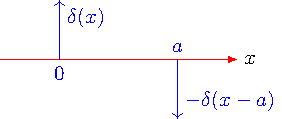
\includegraphics{January2021/4-1.pdf}
\end{center}

}

\sol{

We can solve this problem by dividing the $x$-axis into three portions, within which the particle is free:
\begin{align}
    \psi(x) = \begin{cases}
        e^{ikx} + A e^{-ikx} & x < 0 \\
        B e^{ikx} + C e^{-ikx} & 0 < x < a \\
        D e^{ikx}
    .\end{cases}
\end{align}
The coefficients are determined via boundary conditions:
\begin{align}
    \psi(0^{-}) = \psi(0^{+}) &\Rightarrow 1 + A = B + C \\
    \psi'(0^{+}) - \psi(0^{-}) = \frac{2 m \alpha}{\hbar^2} \psi(0) &\Rightarrow ik\Big[ (B - C) - (1 - A) \Big] = \frac{2 m \alpha}{\hbar^2} (1 + A) \\
    \psi(a^{-}) = \psi(a^{+}) &\Rightarrow B e^{ika} + C e^{-ika} = D e^{ika} \\
    \psi'(0^{+}) - \psi(0^{-}) = -\frac{2 m \alpha}{\hbar^2} \psi(0) & \Rightarrow ik \Big[ D e^{ika} - ( B e^{ika} - C e^{-ika} ) \Big] = -\frac{2 m \alpha}{\hbar^2} D e^{ika}
.\end{align}
The problem asks for the reflection coefficient, which is given as $R = |A|^2$, so we care only to solve the system for $A$.
Unfolding the system of equations and defining $\lambda = 2 m \alpha / (\hbar^2 k)$, we have
\begin{align}
    D &= \frac{1}{1 + i \lambda} ( B - C e^{-2 i k a} ) \nonumber \\
    C &= -\frac{i \lambda}{2 + i \lambda} e^{2 i k a} B \nonumber \\
    B &= \frac{2 + i \lambda}{2 + i \lambda ( 1 + e^{2 i k a} )} [ (1 - i \lambda) - (1 + i \lambda) A ] \nonumber \\
    A &= -\frac{i \lambda [ (2 + i \lambda) e^{2 i k a} + (2 - i \lambda) ]}{(2 + i \lambda)^2 + \lambda^2 e^{2 i k a}}
.\end{align}
Thus, the reflection coefficient
\begin{align}
    \eqbox{ R = \frac{2[ (4 + \lambda^2) + (4 - \lambda^2) \cos(2ka) - 4 \lambda \sin(2ka) ]}{\lambda^4 + (4 + \lambda^2)^2 + 2\lambda^2 [ (4 - \lambda^2) \cos(2 k a) + 4 \lambda \sin(2 k a) ]} }
.\end{align}

(b) Finally, particles are not reflected when
\begin{gather}
    (4 + \lambda^2) + (4 - \lambda^2) \cos(2ka) - 4 \lambda \sin(2ka) = 0 \nonumber \\
    4 - (4 - \lambda^2) \sin^2(ka) - 2 \lambda \sin(2ka) = 0 \nonumber \\
    4 \cos^2(ka) - 4 \lambda \sin(ka) \cos(ka) + \lambda^2 \sin^2(ka) = 0 \nonumber \\
    ( 2 \cos(ka) - \lambda \sin(ka) )^2 = 0 \nonumber \\
    \eqbox{ \tan(ka) = \frac{\hbar^2 k}{m \alpha} }
.\end{gather}
This is a transcendental equation for $k$ and thus there does not exist a closed form for $k$, but we could define $z = ka$ and solve numerically the equation
\begin{align}
    \tan(z) = z/z_0
,\end{align}
where $z_0 = m a \alpha / \hbar^2$.
Observe that there will be an infinite number of solutions, all within the intervals $[n \pi, (n+1/2)\pi]$ (where $n = 0,1,\hdots$), and as $k \rightarrow \infty$ we have $z \rightarrow (2n + 1/2) \pi$.

}


\prob{4.2}{

The purpose of this exercise is to prove what is known as the Hellmann-Feynman theorem.
That theorem relates the derivative of the total energy with respect to a parameter to the expectation value of the derivative of the Hamiltonian with respect to the same parameter.

Consider a time-independent system where:
(1) $\hat{H}_\lambda$ is a Hamiltonian depending upon a continuous parameter $\lambda$, (2) $\ket{\Psi_\lambda}$ is an eigenstate of the Hamiltonian $\hat{H}_{\lambda}$, and (3) $E_{\lambda}$ is the energy of the state $\ket{\Psi_\lambda}$, i.e. $\hat{H}_{\lambda} \ket{\Psi_\lambda} = E_\lambda \ket{\Psi_\lambda}.$

\begin{parts}
    \item Show that:
    \begin{align*}
        \dv{E_{\lambda}}{\lambda} = \bra{\Psi_\lambda} \dv{\hat{H}_\lambda}{\lambda} \ket{\Psi_\lambda}
    .\end{align*}

    \item For a general time-dependent wave function satisfying the time-dependent \\ Schr\"{o}dinger equation the Hellman-Feynman theorem is not valid.
    However show that the following identity holds:
    \begin{align*}
        \bra{\Psi_\lambda} \dv{\hat{H}_\lambda}{\lambda} \ket{\Psi_\lambda} = i \hbar \pdv{t} \bra{\Psi_\lambda(t)}\ket{\dv{\Psi_\lambda(t)}{t}}
    \end{align*}
\end{parts}

}

\sol{

(a) An energy eigenstate of the Hamiltonian satisfies the equation $H \ket{\psi} = E \ket{\psi}$, where the dependence on $\lambda$ is implied for brevity.
Notice then that
\begin{align}
    E = \mel{\psi}{H}{\psi}
,\end{align}
so the derivative
\begin{align}
    \dv{E}{\lambda} &= \dv{\bra{\psi}}{\lambda} H \ket{\psi} + \mel{\psi}{\dv{H}{\lambda}}{\psi} + \bra{\psi} H \dv{\ket{\psi}}{\lambda} \nonumber \\
    &= E_\lambda \underbrace{ \dv{\lambda} \ip{\psi}{\psi} }_{=0} + \mel{\psi}{\dv{H}{\lambda}}{\psi} = \mel{\psi}{\dv{H}{\lambda}}{\psi}
\end{align}

(b) In this part, the relevant equation is the time-dependent Schr\"{o}dinger equation: $i \hbar \pdv*{\ket{\Psi}}{t} = H \ket{\Psi}$.
Thus,
\begin{gather}
    \dv{\lambda} \Big[ \bra{\Psi} i \hbar \pdv{\ket{\Psi}}{t} \Big] = \dv{\lambda} \mel{\Psi}{H}{\Psi} \nonumber \\
    i \hbar \dv{\bra{\Psi}}{\lambda} \pdv{\ket{\Psi}}{t} + i \hbar \bra{\Psi} \dv{\lambda} \pdv{\ket{\Psi}}{t} = \dv{\bra{\Psi}}{\lambda} H \ket{\Psi} + \mel{\Psi}{\dv{H}{\lambda}}{\Psi} + \bra{\Psi} H \dv{\ket{\psi}}{\lambda} \nonumber \\
    i \hbar \bra{\Psi} \dv{\lambda} \pdv{\ket{\Psi}}{t} = \mel{\Psi}{\dv{H}{\lambda}}{\Psi} - i \hbar \pdv{\bra{\Psi}}{t} \dv{\ket{\psi}}{\lambda} \nonumber \\
    \mel{\Psi}{\dv{H}{\lambda}}{\Psi} = i \hbar \pdv{t} \bra{\Psi} \dv{\ket{\Psi}}{\lambda}
\end{gather}

}


\prob{4.3}{

The spin component of an electron along the $z$-axis is determined to be $+1/2$.
Another axis $z'$, makes an angle $\theta$ with $z$.
What is,

\begin{parts}
    \item the probability that a projection of the spin along $z'$ is $+1/2$ or $-1/2$ and,

    \item the mean value of the spin component along $z'$ axis?
\end{parts}

}

\sol{

Let us construct the $z'$ axis such that $\vhat{z}' = \sin{\theta} \vhat{x} + \cos{\theta} \vhat{z}$ and therefore 
\begin{align}
    S_{z'} = \sin{\theta} S_x + \cos{\theta} S_z = \frac{\hbar}{2} \begin{pmatrix}
        \cos{\theta} & \sin{\theta} \\
        \sin{\theta} & -\sin{\theta}
    \end{pmatrix} 
.\end{align}
Diagonalizing, we find eigenvalues $\lambda_{\pm} = \pm 1$ and eigenvectors
\begin{align}
    \chi_{\pm} = \frac{\sin{\theta}}{\sqrt{2(1 \mp \cos{\theta})}} \begin{pmatrix}
        1 \\ (-\cos{\theta} \pm 1)/\sin{\theta}
    \end{pmatrix}
.\end{align}
The probability of measuring $\pm 1/2$ for $S_z'$ is just
\begin{align}
    \eqbox{ P(\pm 1/2) = |\ip{\chi_{\pm}}{+}|^2 = \Big| \frac{\sin{\theta}}{\sqrt{2(1 \mp \cos{\theta})}} \Big|^2 = \frac{\sin^2{\theta}}{2(1 \mp \cos{\theta})} }
.\end{align}

(b) The expectation value can be computed in two ways.
First we can write
\begin{align}
    \expval{S_{z'}} = \mel{+}{S_{z'}}{+} = \frac{\hbar}{2} \cos{\theta}
.\end{align}
Second, we also have
\begin{align}
    \expval{S_{z'}} = \frac{\sin^2{\theta}}{2(1 - \cos{\theta})} - \frac{\sin^2{\theta}}{2(1 + \cos{\theta})} = \eqbox{ \frac{\hbar}{2} \cos{\theta} }
\end{align}

}


\prob{4.4}{

A particle of mass $m$ is in a 1d infinite potential well of width $L$ so that $U(x) = 0$ at $0 < x < L$ and $U(x) = \infty$ outside the well.
The initial state of the particle at $t = 0$ is described by the normalized wave function:
\begin{align*}
    \psi_0(x) = \frac{\sqrt{30}}{L^{5/2}} (L - x) x, \quad 0 < x < L
,\end{align*}
and $\psi_0(x) = 0$ outside the well.

\begin{parts}
    \item Write down the wave function $\psi(x,t)$ at $t > 0$.

    \item Calculate the probabilities $w_n$ or measuring different energies $E_n$ of the particle in the well and show that $\sum_{n=1}^{\infty} w_n = 1$.

    \item Calculate the expectation value of energy.
\end{parts}

\textbf{Hint}: You may need the formulas:
\begin{gather*}
    \int_0^1 z(1-z) \sin(\pi n z) \dd{z} = \frac{2}{\pi^3 n^3} [ 1 - (-1)^n ], \quad n = 1,2,3,\ldots \\
    \sum_{k=1}^{\infty} \frac{1}{(2k-1)^6} = \frac{\pi^6}{960}, \quad \sum_{k=1}^{\infty} \frac{1}{(2k-1)^4} = \frac{\pi^4}{96}
.\end{gather*}

}

\sol{

(a) Recall the spectrum of the infinite square well:
\begin{align}
    \psi_{n}(x) = \sqrt{\frac{2}{L}} \sin(\frac{n \pi x}{L}), \quad E_n = \frac{n^2 \hbar^2 \pi^2}{2 m L^2}
.\end{align}
We can expand any function in the basis of eigenstates as follows
\begin{align}
    \Psi(x,0) = \sum_{n} c_n \psi_n(x)
,\end{align}
where
\begin{align}
    c_n &= \int_{0}^{L} \dd{x} \psi_n^{*}(x) \Psi(x,0) \nonumber \\
    &= \sqrt{\frac{2}{L}} \frac{\sqrt{30}}{L^{5/2}} \int_{0}^{L} \dd{x} x (L - x) \sin(\frac{n \pi x}{L}) \nonumber \\
    &= \sqrt{60} \int_{0}^{1} \dd{z} z(1 - z) \sin(n \pi z) = \frac{2 \sqrt{60}}{\pi^{3} n^3} [1 - (-1)^{n}]
,\end{align}
which is zero for even $n$.
From the expansion at $t = 0$
\begin{align}
    \eqbox{ \Psi(x,t) = \sum_{n} c_n \psi_n(x) e^{-i E_n t / \hbar} = \frac{8}{\pi^3} \sqrt{\frac{30}{L}} \sum_{n={\rm odd}} \frac{1}{n^3} \sin(\frac{n \pi x}{L}) e^{-i E_n t / \hbar} }
.\end{align}

(b) The weights are simply
\begin{align}
    \eqbox{ w_n = |\ip{\psi_n}{\Psi}|^2 = |c_n|^2 = \frac{960}{\pi^2 n^6} }
.\end{align}
Using this, we have
\begin{align}
    \sum_{n={\rm odd}} = \frac{960}{\pi^2} \sum_{n={\rm odd}} \frac{1}{n^6} = 1
,\end{align}
from the hint above.


(c) Finally, the expected value of energy
\begin{align}
    \eqbox{ E_n = \sum_n w_n E_n = \frac{\pi^2 \hbar^2}{2 m L^2} \frac{960}{\pi^6} \sum_{n={\rm odd}} \frac{1}{n^4} = \frac{5 \hbar^2}{m L^2} = \frac{10}{\pi^2} E_1 }
\end{align}

}